\documentclass[tikz,border=8pt]{standalone}
\usepackage[T1]{fontenc}
\usepackage{tikz}
\usetikzlibrary{arrows.meta,positioning,fit,backgrounds}
\definecolor{blue}{RGB}{34,98,184}
\definecolor{green}{RGB}{45,145,120}
\definecolor{orange}{RGB}{194,115,45}
\definecolor{purple}{RGB}{108,95,178}
\definecolor{textgray}{RGB}{38,45,56}
\tikzset{
  box/.style={draw=#1, fill=#1!8, rounded corners=3pt, thick, align=center,
    minimum width=34mm, minimum height=10mm, text=textgray, font=\sffamily\small},
  small/.style={draw=#1, fill=#1!8, rounded corners=3pt, thick, align=center,
    minimum width=29mm, minimum height=9mm, text=textgray, font=\sffamily\scriptsize},
  arrow/.style={-{Latex[length=2.2mm]}, thick, draw=textgray!70}
}
\begin{document}
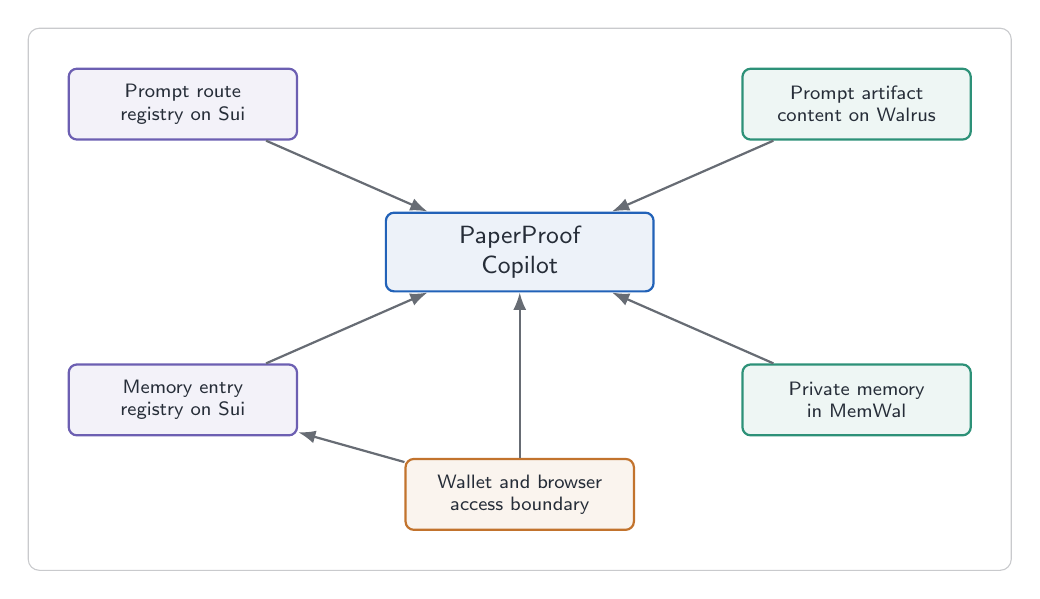
\begin{tikzpicture}[node distance=9mm and 11mm]
  \node[box=blue] (copilot) {PaperProof\\Copilot};
  \node[small=purple, above left=of copilot] (promptreg) {Prompt route\\registry on Sui};
  \node[small=green, above right=of copilot] (promptpkg) {Prompt artifact\\content on Walrus};
  \node[small=purple, below left=of copilot] (memreg) {Memory entry\\registry on Sui};
  \node[small=green, below right=of copilot] (memwal) {Private memory\\in MemWal};
  \node[small=orange, below=21mm of copilot] (wallet) {Wallet and browser\\access boundary};
  \draw[arrow] (promptreg) -- (copilot);
  \draw[arrow] (promptpkg) -- (copilot);
  \draw[arrow] (memreg) -- (copilot);
  \draw[arrow] (memwal) -- (copilot);
  \draw[arrow] (wallet) -- (memreg);
  \draw[arrow] (wallet) -- (copilot);
  \begin{pgfonlayer}{background}
    \node[draw=textgray!25, rounded corners=4pt, fit=(copilot)(promptreg)(promptpkg)(memreg)(memwal)(wallet), inner sep=5mm] {};
  \end{pgfonlayer}
\end{tikzpicture}
\end{document}
